\section{Fakes}

En Fake er en falsk version af en klasses dependancy. Fakes kan bruges når vi ønsker at isolere vores UUT\footnote{Unit Under Test.} fra det systemet som det normalt fungerer i, for at teste isoleteret.

Samtidig kan fakes også bruges i tilfælde af vores dependancies endnu ikke er implementeret.

\paragraph{Dependancies} Da vi ikke kan kontrollere disse externe dependancies, bruges fakes.

\begin{itemize}
	\item \textbf{Eksternal dependancy} - Et objekt i systemet som vores UUT interagerer med, og som vi ikke kontrollerer: \textit{filsystemer, tråde, tid osv.}
	\item \textbf{Internal dependancy} - Et 
\end{itemize}

\subsection{Hvordan bruges Fakes?}

\begin{itemize}
	\item Identificér afhængigheder.
	\item Lav interfaces til dem
	\item Brug \textit{dependency-injection}\footnote{Constructor- eller propertyinjection.}.
\end{itemize}

\subsection{Test typer}
Der findes to typer af Unit tests:

\paragraph{State-Based tests} Vi tester om UUT er i den forventede state efter behandling. Fakes til denne type af test er en \textit{stub}. \\

\textit{''In a state-based test, the assertion is \textbf{ALWAYS} on the UUT, \textbf{NEVER} on the fake(s).}

\paragraph{Interaction-Based} Det testes om UUT har den ønskede adfærd efter behandling. Her kigges der på UUT's adfærd med dens dependencies. Fakes til denne type af test er en \textit{mock}.\\

\textit{''In a Interaction-based test, the assertion is \textbf{ALWAYS} on the mock, \textbf{NEVER} on the UUT.}

\subsection{Fake typer}
Om det er \textit{state-based} eller \textit{interaction-based test} vi laver så vil vi bruge forskellige typer af fakes.

\subsubsection{Stubs}
Stubbe eksisterer kun for at give UUT de dependancies den behøver for at fungere.
Hvis en klasse Calculator er afhængig af en klasse der skal lave beregninger, kan der laves en stub af denne klasse, der blot returnerer en fastlagt værdi.

\paragraph{Procedure for stubbe} Assert sker på UUT og \textit{ikke} på selve stubben. En stub kan derfor ikke være skyld i at en test fejler.

\begin{itemize}
	\item \textbf{Arrange} - Opsætning af UUT og dens dependancies.
	\item \textbf{Act} - Stimuler UUT'en. Få den til at gøre som vi ønsker.
	\item \textbf{Assert} - Assert at vi får det ønskede resultat, altså om UUT's state er den ønskede.
\end{itemize}

%\begin{figure}
%	\centering
%	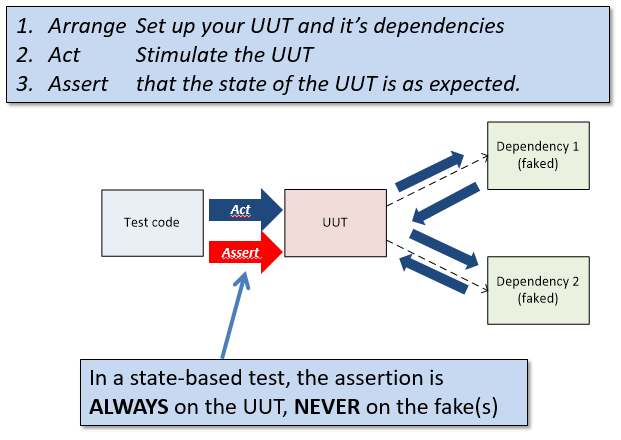
\includegraphics[width=0.7\linewidth]{figs/stubTest.PNG}
%	\caption{Unit testing med stubbe.}
%	\label{fig:stubTest}
%\end{figure}

For klassediagrammet på figur~\ref{fig:stubNoInterface} ønsker vi at lave en \textit{state-based test} på klassen A. Klassen har en afhængighed, Klassen B.

\begin{figure}[H]
	\centering
	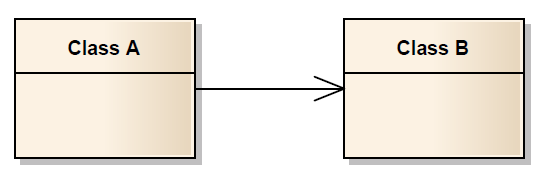
\includegraphics[width=0.5\linewidth]{figs/stubNoInterface.PNG}
	\caption{Afhængighed - DIP ikke opfyldt.}
	\label{fig:stubNoInterface}
\end{figure}

Brugen af et interface vil her give mening. Vi påfører DIP of får da:

\begin{figure}[H]
	\centering
	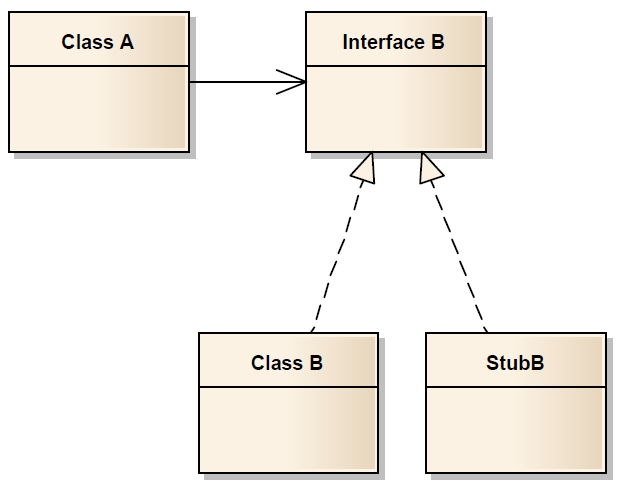
\includegraphics[width=0.55\linewidth]{figs/stubInterface.PNG}
	\caption{Klassediagram for brug af stub.}
	\label{fig:stubInterface}
\end{figure}

Her laves en en stub af interfacet B, hvorefter man kan bruge stubben til at teste UUT i et kontrolleret miljø.

\paragraph{Constructor injection}
Stubbe handler om at teste stadier. Det kan da være en fordel at anvende constructor injection.

\subsubsection{Mocks}
Mocks bruges til adfærdsbaserede tests, hvilket betyder at vi ikke tester på UUT. Her testes i stedet på Mock'en, efter vi har \textit{''act'et''} på UUT.

\begin{figure}[H]
\centering
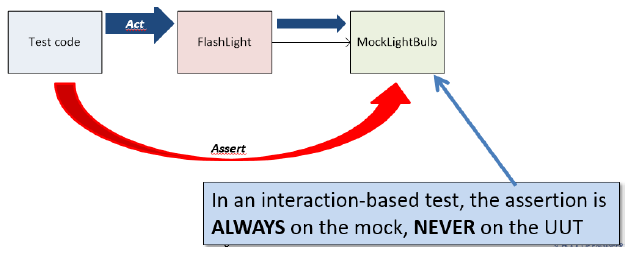
\includegraphics[width=0.9\linewidth]{figs/mockTest.PNG}
\caption{Unit testing med mock}
\label{fig:mockTest}
\end{figure}

Da der med Mocks, testes om UUT har foretaget de forventede operationer på dens dependencies, bliver mock-klassen nødt til at recorde om operationen er sket.

\paragraph{Procedure for stubbe} Det er i modsætning til stubbe, muligt for en mock at få en test til at fejle.

\begin{itemize}
	\item Arrange - Opsætning af UUT og dens dependancies.
	\item Act - Stimuler UUT'en. Få den til at gøre det vi ønsker.
	\item Assert - Assert på om mock klassen blev interageret med korrekt af UUT.
\end{itemize}

Da en mock skal indeholde nogle recordings er en mock typisk mere tidskrævende at skrive, og samtidig sværere at genbruge.

\vskip.3cm

\begin{lstlisting}[caption=Eksempel på en mock.,label=code:mock]
public class FakeWebService : IWebService
{
	public string LastError;
	
	public void LogError(string message)
	{
		LastError = message;
	}
}
\end{lstlisting}

\subsection{Isolation Frameworks}

NSubstitute er et isolation framework, som kan oprette fakes på baggrund af interfaces. I NSubstitute kan vi asserte på resultat af et funktionskald (Stubs) eller om en funktion i en mock er blevet kaldt med \textit{recieved()}.

\subsubsection{Brug af NSubstitute}

Eksemplet i Code listing~\ref{code:nsub} bruger \textit{Calculator} et interface til \textit{IAdditionCalculator}, som står for addering af tal.\\

Eksemplet viser en \textbf{adfærdsbaseret test} (linjer 15-21) hvor vi \textit{asserter} implicit på vores \textbf{mock}, \textit{\_fakeAdditionCalculator}.\\

I linjerne 23-30 bruges den samme fake til \textbf{tilstandsbaseret test}, da selve \textit{assert} sker på \textit{\_uut}.

\vskip.3cm

\begin{lstlisting}[caption=Eksempel på fakes med NSubstitute.,label=code:nsub,morekeywords={Calculator,IAdditionCalculator}]
[TestFixture]
public class CalculatorTestUnit
{
	Calculator _uut;
	private IAdditionCalculator _fakeAdditionCalculator;
	
	[SetUp]
	public void Setup()
	{
		// setup af fake
		_fakeAdditionCalculator = Substitute.For<IAdditionCalculator>();
		_uut = new Calculator(_fakeAdditionCalculator);
	}
	
	[Test]
	public void Add_Adding1And2_SubclassReceivedCall()
	{
		// fake bruges som mock, med implicit assertion
		_uut.Add(1,2);
		_fakeAdditionCalculator.Received().Add(1, Arg.Any<int>());
	}
	
	[Test]
	public void Add_Adding1And2_Returns3()
	{
		// fake bruges som stub
		_fakeAdditionCalculator.Add(1, 2).Returns(3);
		Assert.That(_uut.Add(1, 2), Is.EqualTo(3));
	}
}
\end{lstlisting}
